\chapter{深度生成模型}
\label{cha:gen}

在机器学习中,数据的合成与采样是一类重要的研究课题。
它的基本目标是:按照训练数据的分布规律进行采样,生成一系列相似的新样本,
即使得模型的概率分布 $\PMODEL(\bm x)$ 尽可能的接近训练数据的概率分布 $\PDATA(\bm x)$:
\begin{align}
	\PMODEL(\bm x) \approx \PDATA(\bm x) \label{eq:densityestimation}
\end{align}
数据的概率分布 $\PDATA(\bm x)$ 通常不会显式地给出,而是在训练数据集中以采样的形式间接提供。
而深度生成模型,顾名思义,正是使用深度学习解决此类问题的有效手段。


\begin{figure}[h]
	\centering%
	{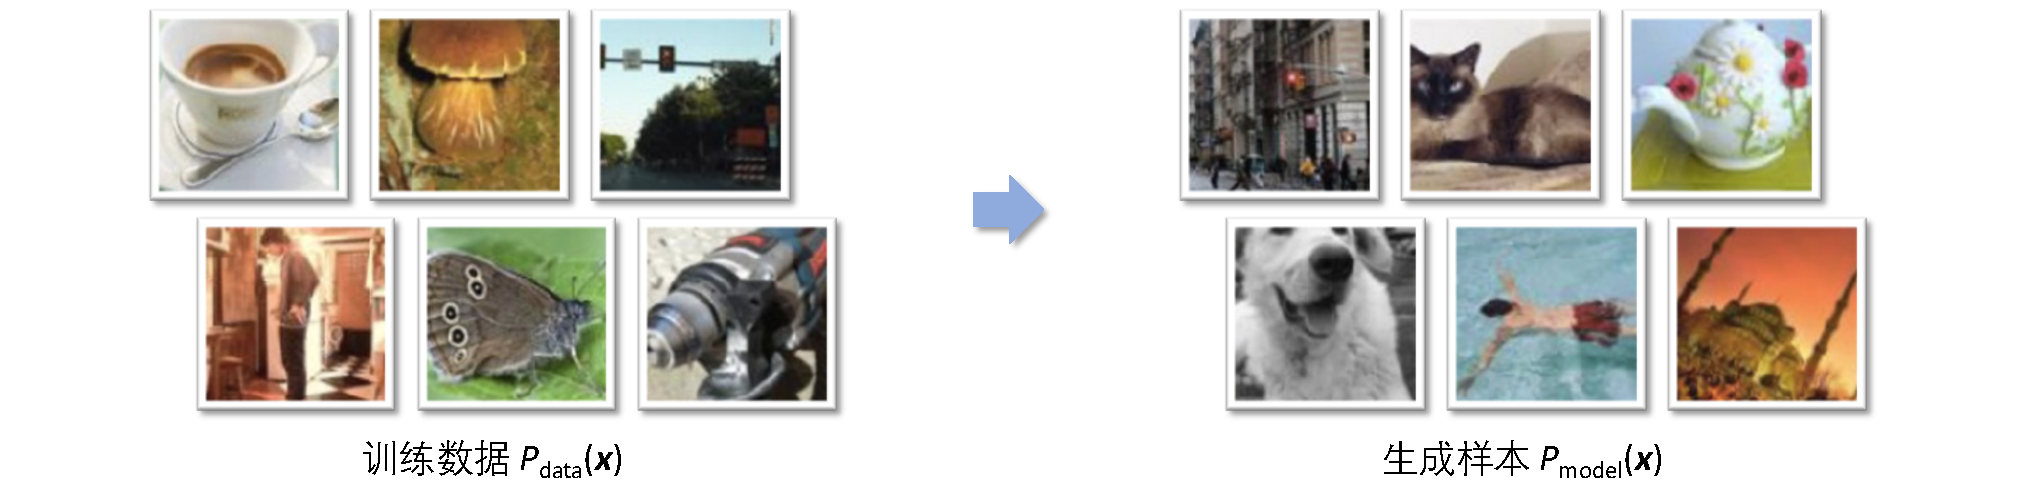
\includegraphics[width=.99\textwidth]{imggen}}
	\caption{图像生成问题\cite{gantutorial}}\label{fig:imggen}
\end{figure}

合成与采样任务通常对数据的形式没有任何假设,
因此,其外延涵盖了图像生成、视频生成、文本生成、语音生成等各类任务,而不仅仅局限于图像生成。
% 它通常一个概率模型 $\PMODEL(\bm x)$,即模型的输出并不是一成不变的,而具有一定的随机性。
但是,为了简单起见,本章仅仅以图像生成为例,讲解深度生成模型的原理与方法。
如果不加以特殊说明,在本章中深度生成模型均指代图像的深度生成模型%,而在 \ref{section:gen3d} 节中均指代点云的深度生成模型
。

\section{深度生成模型的分类}
深度生成模型所求解的 \eqref{eq:densityestimation} 实际上是无监督学习中的密度估计问题。按照是否显式地定义并优化
$\PMODEL(\bm x)$,主要的方法被分为两大类:
\begin{itemize}
	\item 显式密度估计:显式的定义模型的分布 $\PMODEL(\bm x)$,且此定义参与优化过程;
	\item 隐式密度估计:给出可按分布 $\PMODEL(\bm x)$ 采样的模型,但 $\PMODEL(\bm x)$ 没有被显式定义,也不直接参与优化过程。
\end{itemize}
\begin{figure}[h]
	\centering%
	{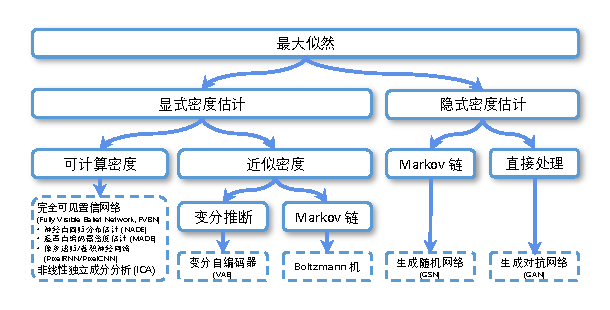
\includegraphics[width=.99\textwidth]{gentype}}
	\caption{深度生成模型的分类\cite{gantutorial}}\label{fig:gentype}
\end{figure}
按照模型所使用的密度估计方法以及具体的实现方式,深度生成模型可以被进一步细分\cite{gantutorial},如图 \ref{fig:gentype} 所示。其中,目前最常用的有以下四种:
\begin{itemize}
	\item 变分自编码器\cite{vae} (Variational Autoencoder, VAE);
	\item 生成对抗网络\cite{gan} (Generative Adversarial Network, GAN);
	\item 像素递归神经网络\cite{pixelrnn} (Pixel Recurrent Neural Networks, PixelRNN);
	\item 像素卷积神经网络\cite{pixelcnn} (Pixel Convolutional  Neural Networks, PixelCNN)。
\end{itemize}

本章将主要介绍 VAE 与 GAN。

\section{数学准备}
为了更清楚地阐述本章内容,本节补充介绍一些必要的数学概念。

\subsection{Bayes 公式}
Bayes 公式如 \eqref{eq:bayes} 所示,它表明了后验概率密度 $p(\bm z | \bm x)$、先验概率密度 $p(\bm z)$以及似然函数 $p(\bm x | \bm z)$ 三者间的关系:

\begin{align}
	%p(\bm \theta | \bm x) = \frac{p(\bm x |  \bm \theta) \cdot p(\bm \theta)}{p(\bm x)} \label{eq:bayes}
	p(\bm z | \bm x) = \frac{p(\bm x | \bm z) \cdot p(\bm z)}{p(\bm x)} \label{eq:bayes}
\end{align}
% 其中 $p(\bm \theta | \bm x)$ 为后验概率密度,$p(\bm \theta)$ 为先验概率密度,$p(\bm x | \bm \theta)$ 为似然函数。
% 其中 $p(\bm z | \bm x)$ 为后验概率密度,$p(\bm z)$ 为先验概率密度,$p(\bm x | \bm z)$ 为似然函数。
其中,我们通常把观测量 $\bm x$ 的概率密度 $p(\bm x)$ 视为常数。

% \begin{itemize}
%     \item $p(\bm \theta | x)$ 为后验概率密度;
%     \item $p(x | \bm \theta)$ 为先验概率密度;
%     \item $p(x | \bm \theta)$ 为似然函数。
% \end{itemize}

\subsection{多维正态分布}
多维正态分布又称多维 Gauss 分布,是常用概率分布之一。其参数有两个,分别是期望向量 $\bm \mu$ 和正定对称的协方差矩阵 $\bm \Sigma$。
% 若随机向量 \bm x \sim \NormDist(\bm \mu, \bm \Sigma)$,则
对于 $n$ 维的情况,其概率密度函数为
\begin{align}
	p_{\bm x \sim \NormDist(\bm \mu, \bm \Sigma)}(\bm x) =
	\sqrt{\frac{1}{(2\pi)^n |\bm\Sigma|}} \cdot
	\exp \left(- \frac{1}{2} (\bm x - \bm \mu)^T \Sigma^{-1} (\bm x - \bm \mu)\right)
	\label{eq:normdist}
\end{align}

%(一维)正态分布 $\NormDist(\mu, \sigma^2)$ 即 $\bm \mu = \mu, \bm \Sigma = \sigma^2$ 的多维正态分布。 
\subsection{Kullback-Leibler (KL) 散度与 Jensen–Shannon (JS) 散度}
要衡量两个概率分布 $p(\bm x)$ 与 $q(\bm x)$ 的差异程度,我们可以使用散度。

在统计学中,
散度 $\Div{\cdot}{\cdot}$ 是一个泛函,其输入为两个
%同支撑集的
概率密度函数 $p(\bm x)$ 与 $q(\bm x)$,输出为一个实数,且满足
\begin{itemize}
	\item $\Div{p}{q} \ge 0, \quad  \forall p, q$;
	\item $\Div{p}{q} = 0 \, \Leftrightarrow \, p(\bm x) = q(\bm x), \, \text{  a. e.}$。
\end{itemize}
可以证明:
\begin{align}
	\DKL{p}{q} & = \EXPECT{\bm x \sim p}{\left[ {\log \frac{p(\bm x)}{q(\bm x)}} \right]} \label{eq:kldiv} \\
	\DJS{p}{q} & =
	\frac{1}{2}\, \DKL*{p}{\frac{p + q}{2}} +
	\frac{1}{2}\, \DKL*{q}{\frac{p + q}{2}} \label{eq:jsdiv}
\end{align}
都满足散度定义,因此我们把 \eqref{eq:kldiv} 称为 KL 散度,把 \eqref{eq:jsdiv} 称为 JS 散度。

值得注意的是,虽然 JS 散度是对称的,但 KL 散度却不对称,即:
$\forall p, q, \DJS{p}{q} = \DJS{q}{p}$;$\exists p, q, \DKL{p}{q} \ne \DKL{q}{p}$。%因此,我们不可以将 KL 散度称为两概率分布间的“距离”。
因此,计算 KL 散度时一定不能混淆两概率分布的先后顺序。




\subsection{$K$-Lipschitz 连续 与 Lipschitz 常数}
若函数 $f: \mathbb{R}^n \to \mathbb{R}$ 满足
\begin{align}
	\Norm*{f\left( \bm x_1 \right)-f\left( \bm x_2 \right)} \leq K \cdot \Norm*{\bm x_1-\bm x_2}
	\label{eq:lip}
\end{align}
则称其是 $K$-Lipschitz 连续的。满足 \eqref{eq:lip} 的最小 $K$ 称为函数 $f$ 的 Lipschitz 常数,记为
$\Norm{f}_{\mathrm{Lip}}$。











\section{引入:自编码器 (Autoencoder, AE) \label{section:ae}}
自编码器是用于提取数据低维特征的有力武器,其架构如图 \ref{fig:ae} 所示。

\begin{figure}[h]
	\centering%
	{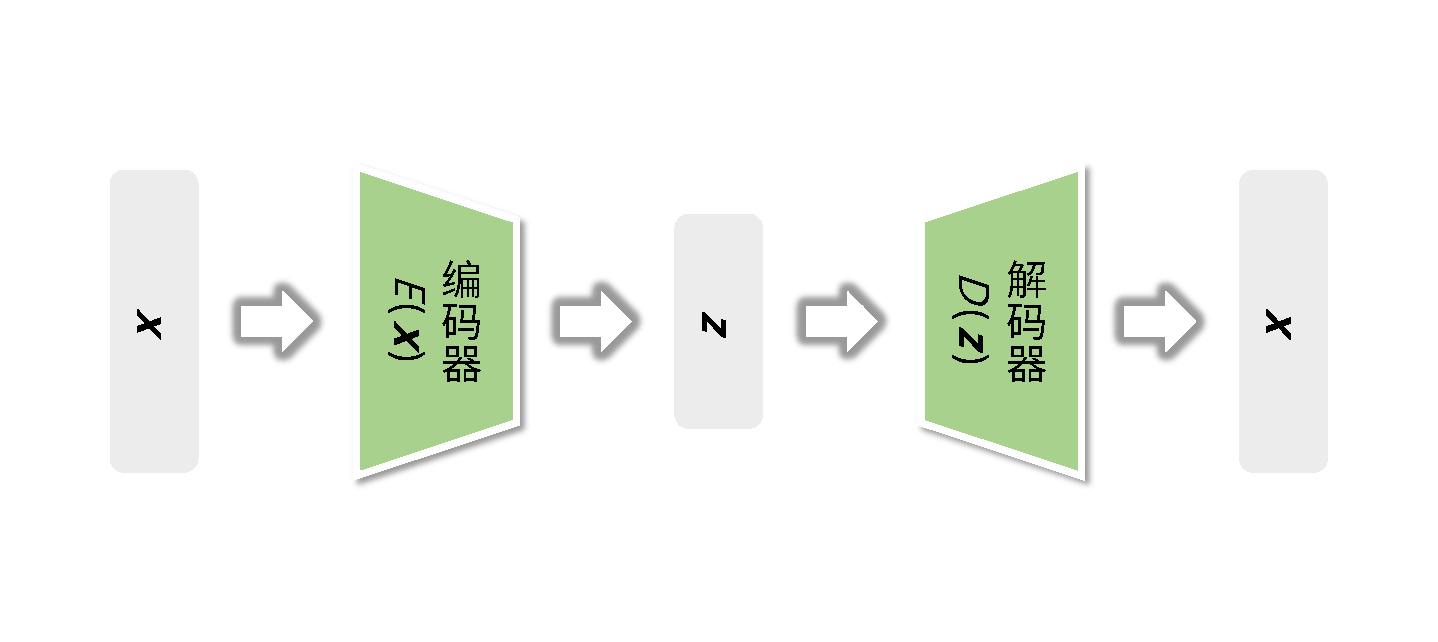
\includegraphics[width=.99\textwidth]{ae}}
	\caption{自编码器}\label{fig:ae}
\end{figure}

自编码器通常包括编码器 $E$、一个解码器 $D$ 和一个隐表示层 $\bm z$。
对于任意的数据 $\bm x$,编码器首先将其编码为隐向量 $\bm z = E(\bm x; \bm\theta_E)$。
随后,解码器对其进行重建 $\bm {\hat x} = D(\bm z; \bm\theta_D)$。
自编码器的目标是通过最小化重建误差
\begin{align}
	\Loss(\theta_E, \theta_D) = \sum_k \Norm{\bm  x_k - \bm {\hat x}_k}^2 \label{eq:aeloss}
\end{align}
来确保输入数据 $\bm x$ 能够尽可能地被编码且准确恢复。其中 $k$ 表示训练数据的编号。

通常来说,$\bm z$ 的维度要远远低于 $\bm x$,因为
这样的设计会强制自编码器捕获到数据最显著的差异,亦即特征,而忽略掉无意义的信息。
否则,如果 $\bm z$ 的维度与 $\bm x$ 的维数持平或者更高,则自编码器不会主动的完成特征提取的任务。

自编码器是一种无监督的方法,即不必提供成对的标注数据,即可完成低维特征的提取。
虽然它不是一个深度生成模型,但它启发了深度生成模型 VAE 的设计。
我们将在第 \ref{section:vae} 节简要介绍它。

















\section{变分自编码器 (Variational Autoencoder, VAE) \label{section:vae}}
与自编码器类似,VAE\cite{vae} 的基本想法是:假设数据 $\bm x $ 是根据一个不可见的隐向量 $\bm z \sim \NormDist(\bm 0, \bm I)$,按照概率 $p(\bm x | \bm z; \bm \theta)$ 生成出来的:
\begin{align}
	\PMODEL(\bm x; \bm\theta) = \int_{\bm z} p(\bm x | \bm z; \bm\theta) \cdot p(\bm z) \cdot d\bm{z} \label{eq:vaepmodel}
\end{align}
% 与自编码器类似,\eqref{eq:vaepmodel} 中的似然函数 $p(\bm x | \bm z; \bm\theta)$ 也被称为解码器网络。
其中的似然函数 $p(\bm x | \bm z; \bm\theta)$ 也被称为解码器网络,与自编码器的命名方式类似。


根据最大似然估计,为了%尽量
尽可能满足 \eqref{eq:densityestimation},我们需要求出网络参数 $\bm\theta$ 来最大化 $\log \PMODEL(\bm x; \bm\theta)$。
但稍加分析,我们就会发现,数据似然函数 $\PMODEL(\bm x; \bm\theta)$ 与后验分布 $p(\bm z | \bm x; \bm\theta)$ 均不能有效计算,因此我们要另辟蹊径。

文献 \inlinecite{vae} 提出了一个创造性的想法:用一个新的编码器网络 $q(\bm z | \bm x; \bm\phi)$ 来近似不能有效计算的后验分布 $p(\bm z | \bm x; \bm\theta)$。
% 这使得我们可以推导出一个变分下界,让问题变得可解。
稍加分析,我们就会发现:
\begin{align}
	\,       & \log \PMODEL(\bm x; \bm \theta)               &                                                           & \notag \\
	= \,     & \EXPECT{\bm z \sim q(\bm z | \bm x; \bm\phi)}
	{\left[\log \PMODEL(\bm x; \bm\theta)\right]}
	         &                                               & \text{$\PMODEL(\bm x; \bm\theta)$ 与 $\bm z$ 无关} \notag          \\
	= \,     & \EXPECT{\bm z \sim q(\bm z | \bm x; \bm\phi)}
	{\left[
			\log\frac{p(\bm x | \bm z; \bm\theta) \cdot p(\bm z)}{p(\bm z | \bm x; \bm\theta)}
	\right]} &                                               & \text{Bayes 公式 \eqref{eq:bayes}}\notag                           \\
	= \,     &
	\EXPECT{\bm z} {\left[
			\log\frac{q(\bm z | \bm x; \bm\phi)}{p(\bm z | \bm x; \bm\theta)}
			\right]}
	+
	\EXPECT{\bm z} {\left[\log p(\bm x | \bm z; \bm\theta)\right]}
	-
	\EXPECT{\bm z} {\left[\log
			\frac{q(\bm z | \bm x; \bm\phi)}{p(\bm z)}
	\right]} &                                               & \text{对数运算;期望可加}\notag                                    \\
	= \,     &
	\underbrace{\DKL{q(\bm z | \bm x; \bm\phi)}{p(\bm z | \bm x; \bm\theta)}}_{\ge 0}
	\notag                                                                                                                        \\
	\,       &
	\quad \quad
	+ \underbrace{
		\EXPECT{\bm z} {\left[\log p(\bm x | \bm z; \bm\theta)\right]}
		- \DKL{q(\bm z | \bm x; \bm\phi)}{p(\bm z)}}_{\Loss(\bm \phi, \bm\theta)}
	         &                                               & \text{KL 散度的定义\eqref{eq:kldiv}}\notag                         \\
	\ge      & \,\Loss(\bm \phi, \bm \theta) \notag
\end{align}
即 $\Loss(\bm \phi, \bm \theta)$ 一定不会超过对数似然函数 $\log \PMODEL(\bm x; \bm\theta)$ 的值:
\begin{align}
	\Loss(\bm \phi, \bm\theta) =
	\underbrace{\EXPECT{\bm z} {\left[\log p(\bm x | \bm z; \bm\theta)\right]}}
	_{\text{重建损失函数}}
	-
	\underbrace{\DKL{q(\bm z | \bm x; \bm\phi)}{p(\bm z)}}
	_{\text{KL 损失函数}}
	\le \log\PMODEL(\bm x; \bm\theta)
	\label{eq:ELBO}
\end{align}
因此,我们将 $\Loss(\bm \phi, \bm \theta)$ 称为变分下界 (Variational Lower Bound, Evidence Lower Bound, ELBO)。

要最大化对数似然 $\log \PMODEL(\bm x; \bm\theta)$,我们可以通过最大化变分下界 $\Loss(\bm \phi, \bm \theta)$ 来间接地实现。那么,$\Loss(\bm \phi, \bm \theta)$ 是否可以被有效计算呢?答案是肯定的。

变分下界 $\Loss(\bm \phi, \bm \theta)$ 中的第一项 $\EXPECT{\bm z} {\left[\log p(\bm x | \bm z; \bm\theta)\right]}$ 通常被称为重建损失函数,它可以通过对 $\bm z \sim q(\bm z | \bm x; \bm\phi)$ 采样,然后计算解码器网络输出 $p(\bm x | \bm z; \bm\theta)$ 的方式求出。如果我们进一步假设解码器网络 $p(\bm x | \bm z; \bm\theta) = \NormDist\left(\bm \mu_\theta(\bm z; \bm \theta), \sigma^2 I\right)$ %为各向同性且方差固定的多维高斯分布
,那么根据 \eqref{eq:normdist},重建误差即
\begin{align}
	{%\EXPECT{\bm z}
		{%\left[
				\log p(\bm x | \bm z; \bm\theta)%\right]
			}}
	 & =
	\underbrace{\left[ - \frac{n}{2} \cdot \log\left(2\pi\sigma^2\right) \right]}_{C}
	-
	\underbrace{\left[ \frac{1}{2\sigma^2} \right]}_{\lambda} \cdot \Norm*{\bm x - \bm \mu_\theta(\bm z; \bm \theta)}^2 \notag \\
	 & = - \lambda \cdot\Norm*{\bm x - \bm \mu_\theta(\bm z; \bm \theta)}^2 + C
	\label{eq:vaerecons}
\end{align}
其中超参数 $\lambda = 1/\left(2\sigma^2\right)> 0$。这与自编码器的损失函数 \eqref{eq:aeloss} 如出一辙。

变分下界 $\Loss(\bm \phi, \bm \theta)$ 中的第二项 $\DKL{q(\bm z | \bm x; \bm\phi)}{p(\bm z)}$ 通常被称为 KL 损失函数,因为它希望近似的后验分布 $q(\bm z | \bm x; \bm\phi)$ 尽可能接近先验分布 $p(\bm z)$。
如果我们进一步假设近似的后验分布
$q(\bm z | \bm x; \bm\phi) = \NormDist
	\left(
	\bm\mu_{\bm\phi}   (\bm x; \bm\phi),
	\bm\Sigma_{\bm\phi}(\bm x; \bm\phi)
	\right)$,则 KL 损失函数项有闭合解,可被解析地算出。

综上所述,在训练 VAE 时,我们需要最大化其变分下界,即优化以下损失函数:
\begin{align}
	\argmin{\bm\theta, \bm\phi}
	- \Loss(\bm \phi, \bm \theta) & =
	\argmin{\bm\theta, \bm\phi}
	- {\EXPECT{\bm z} {\left[\log p(\bm x | \bm z; \bm\theta)\right]}}
	+ \DKL{q(\bm z | \bm x; \bm\phi)}{p(\bm z)}
	\notag                                                                      \\
	                              & = \argmin{\bm\theta, \bm\phi} \lambda \cdot %\cdot
	{\EXPECT{\bm z}{\left[\Norm*{\bm x - \bm \mu_\theta(\bm z; \bm \theta)}^2\right]}}
	+ \DKL{q(\bm z | \bm x; \bm\phi)}{p(\bm z)}
\end{align}
其中超参数 $\lambda > 0$;而要通过 VAE 生成新样本时,我们按照 \eqref{eq:vaepmodel} 采样就可以了。

VAE 在图像生成任务上的表现如图 \ref{fig:vaeimg} 所示。它的缺点是,生成的图片普遍比较模糊。
\begin{figure}[h]
	\centering%
	{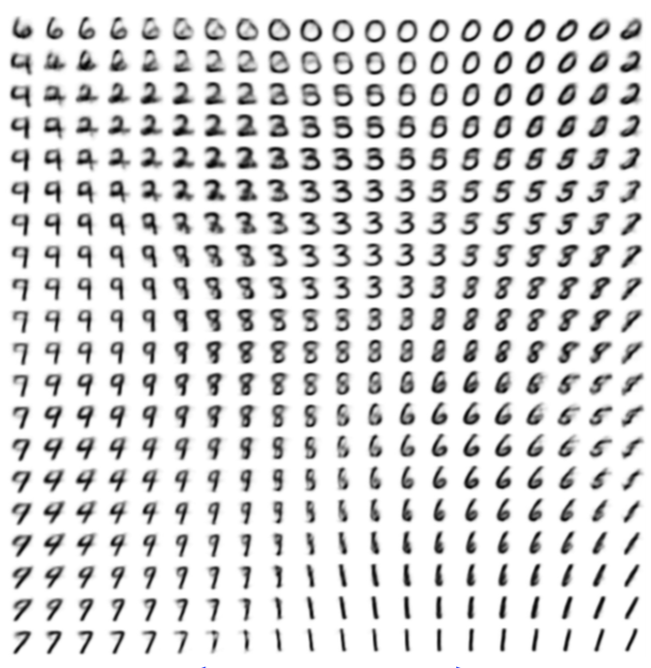
\includegraphics[width=.65\textwidth]{vaeimg}}
	\caption{使用 VAE 解决图像生成任务\cite{vae}}\label{fig:vaeimg}
\end{figure}





% GAN的改进

% WGAN, WGAN-GP
% DRAGAN
% SNGAN

\section{生成对抗网络 (Generative Adversarial Network, GAN) \label{section:gan}}
GAN\cite{gan} 是目前所有的深度生成模型中表现最出色的。图 \ref{fig:gan} 展现了其基本思想和架构。


\begin{figure}[h]
	\centering%
	{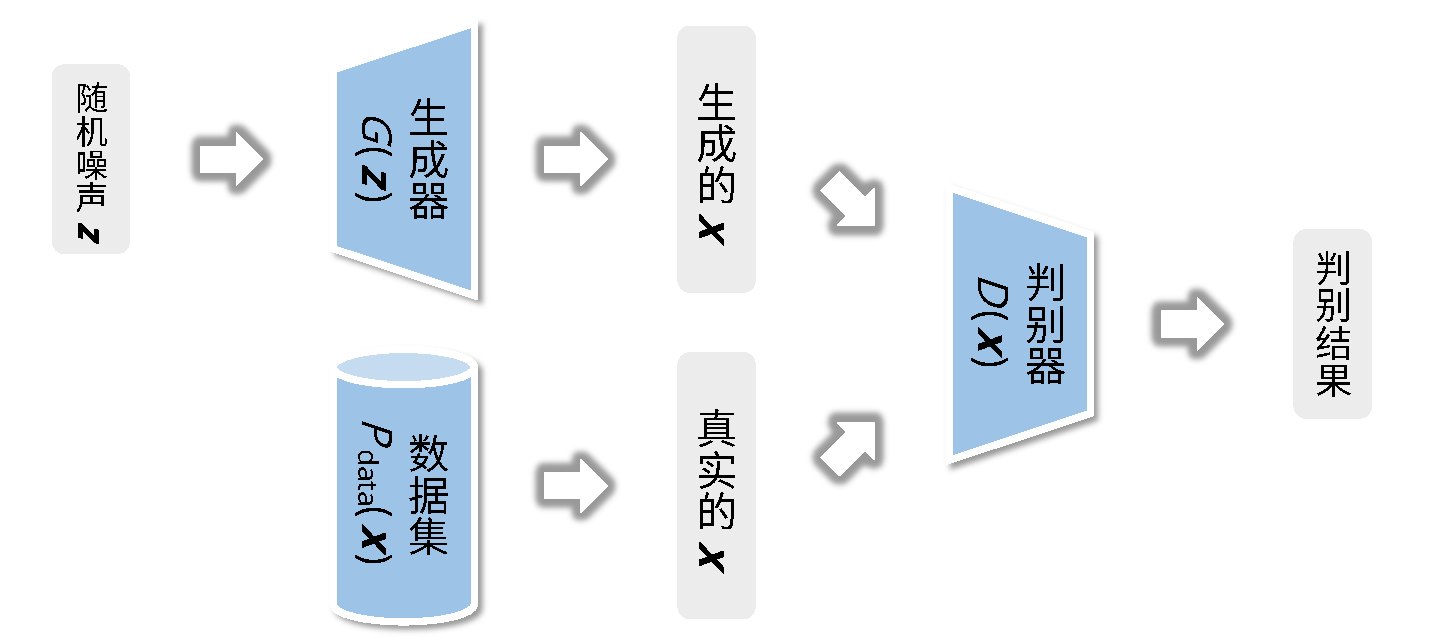
\includegraphics[width=.9\textwidth]{gan}}
	\caption{生成对抗网络}\label{fig:gan}
\end{figure}
%它的基本思想源于
GAN 创造性地将博弈论的概念引入到了深度生成模型中,建立了一个生成器网络 (Generator, $G$) 和 判别器网络 (Discriminator, $D$) 之间的博弈场景:
生成器网络 $G$ 根据隐随机向量 $\bm z \sim \NormDist(\bm 0, \bm I)$ 的观测值直接生成新样本 $\bm x = G(\bm z; \bm\theta_G)$;而判别器网络 $D$ 需要分辩出一个特定的样本是 $G$ 生成的还是训练数据集中已有的。通常,$D$ 通过输出一个概率值 $D(\bm x; \bm\theta_D) \in [0, 1]$ 的形式,来表示它的判定结果。

在这个博弈游戏中,判别器网络 $D$ 的终极目标是
%尽可能的
把 $G$ 生成的样本和数据集中已有的样本区分开,
而生成器网络 $G$ 的终极目标是生成足够接近于训练数据集的新样本,使之无法区分,以欺骗 $D$。
因此,我们可以使用一个零和博弈的过程来训练 $D$ 和 $G$。令 $D$ 的损失为 $\Loss(\bm\theta_G, \bm\theta_D)$:%其中
\begin{align}
	\Loss(\bm\theta_G, \bm\theta_D) =
	- \EXPECT{\bm x \sim \PDATA(\bm x)}           \log(    D(\bm x; \bm\theta_D))
	- \EXPECT{\bm z \sim \NormDist(\bm 0, \bm I)} \log(1 - D( G(\bm z; \bm\theta_G); \bm\theta_D))
	\label{eq:ganloss}
\end{align}
则 $G$ 的损失恰好为其相反数 $- \Loss(\bm\theta_G, \bm\theta_D)$。

在此博弈过程中,$G$ 和 $D$ 都会根据对方的决策来调整自己的决策——网络参数 $\bm \theta_G, \bm \theta_D$,以最小化自己的损失。
文献 \inlinecite{gan} 的分析表明,% 如果游戏的 Nash 均衡点 $\bm\theta_G^*, \bm\theta_D^*$ 存在,
如果 $G, D$ 有无限的表达能力,且 $D$ 可以达到最优状态 $D(\bm x; \bm\theta_D^*) = \PDATA(\bm x)/(\PDATA(\bm x) + \PMODEL(\bm x))$,那么随着训练过程的推进,$G$ 和 $D$ 将收敛于游戏的 Nash 均衡点 $\bm\theta_G^*, \bm\theta_D^*$:
\begin{subequations}
	\begin{align}
		\bm\theta_D^* = & \argmin{\bm\theta_D} \Loss(\bm\theta_G^*, \bm\theta_D)\label{eq:nash1} \\
		\bm\theta_G^* = & \argmax{\bm\theta_G} \Loss(\bm\theta_G, \bm\theta_D^*)\label{eq:nash2}
	\end{align}
\end{subequations}
这时,$G$ 生成的样本变得非常真实,完全不可区分,而 $D$ 也无法对任何输入样本进行判断,处处输出 $D(\bm x; \bm\theta_D) = \frac{1}{2}$。此时,我们就可以丢弃 $D$,直接使用 $G$ 来生成新样本。

为了模拟出上述博弈过程,我们通常先假设对方已经给出最优解,即 $\bm\theta_G = \bm\theta_G^*, \bm\theta_D = \bm\theta_D^*$,然后通过随机梯度下降 (Stochastic gradient descent, SGD) 等优化方法,交替优化式 \eqref{eq:nash1},\eqref{eq:nash2},完成 GAN 的训练。

文献 \inlinecite{gan} 指出:在实际的应用%过程
中,我们通常会使用最小化
$- \log(D( G(\bm z))$
的方式来替代 \eqref{eq:nash2} 中的最大化
$- \log(1 - D( G(\bm z))$ 的过程,因为前者能够再训练初期为 $G$ 提供更强的梯度信息,从而加速收敛过程。

综上所述,要训练 GAN,我们在实践中%实践中会%使用 SGD 等优化方法,
通常会交替最小化以下损失函数:
\begin{subequations}
	\label{eq:ganloss0}
	\begin{align}
		\Loss_D(\bm\theta_D; \bm\theta_G) & =
		- \EXPECT{\bm x \sim \PDATA(\bm x)}           \log(    D(\bm x; \bm\theta_D))
		- \EXPECT{\bm z \sim \NormDist(\bm 0, \bm I)} \log(1 - D( G(\bm z; \bm\theta_G); \bm\theta_D))
		\label{eq:ganloss1}                   \\
		\Loss_G(\bm\theta_G; \bm\theta_D) & =
		- \EXPECT{\bm z \sim \NormDist(\bm 0, \bm I)} \log(D( G(\bm z; \bm\theta_G); \bm\theta_D))
		\label{eq:ganloss2}
	\end{align}
\end{subequations}

GAN 在图像生成任务上的表现非常出色,如图 \ref{fig:ganimg} 所示。除了能生成图像外,GAN 还可以对图像进行插值。如图 \ref{fig:ganinter} 所示。
\begin{figure}[h]
	\centering%
	\subcaptionbox{图像生成\label{fig:ganimg}}
	{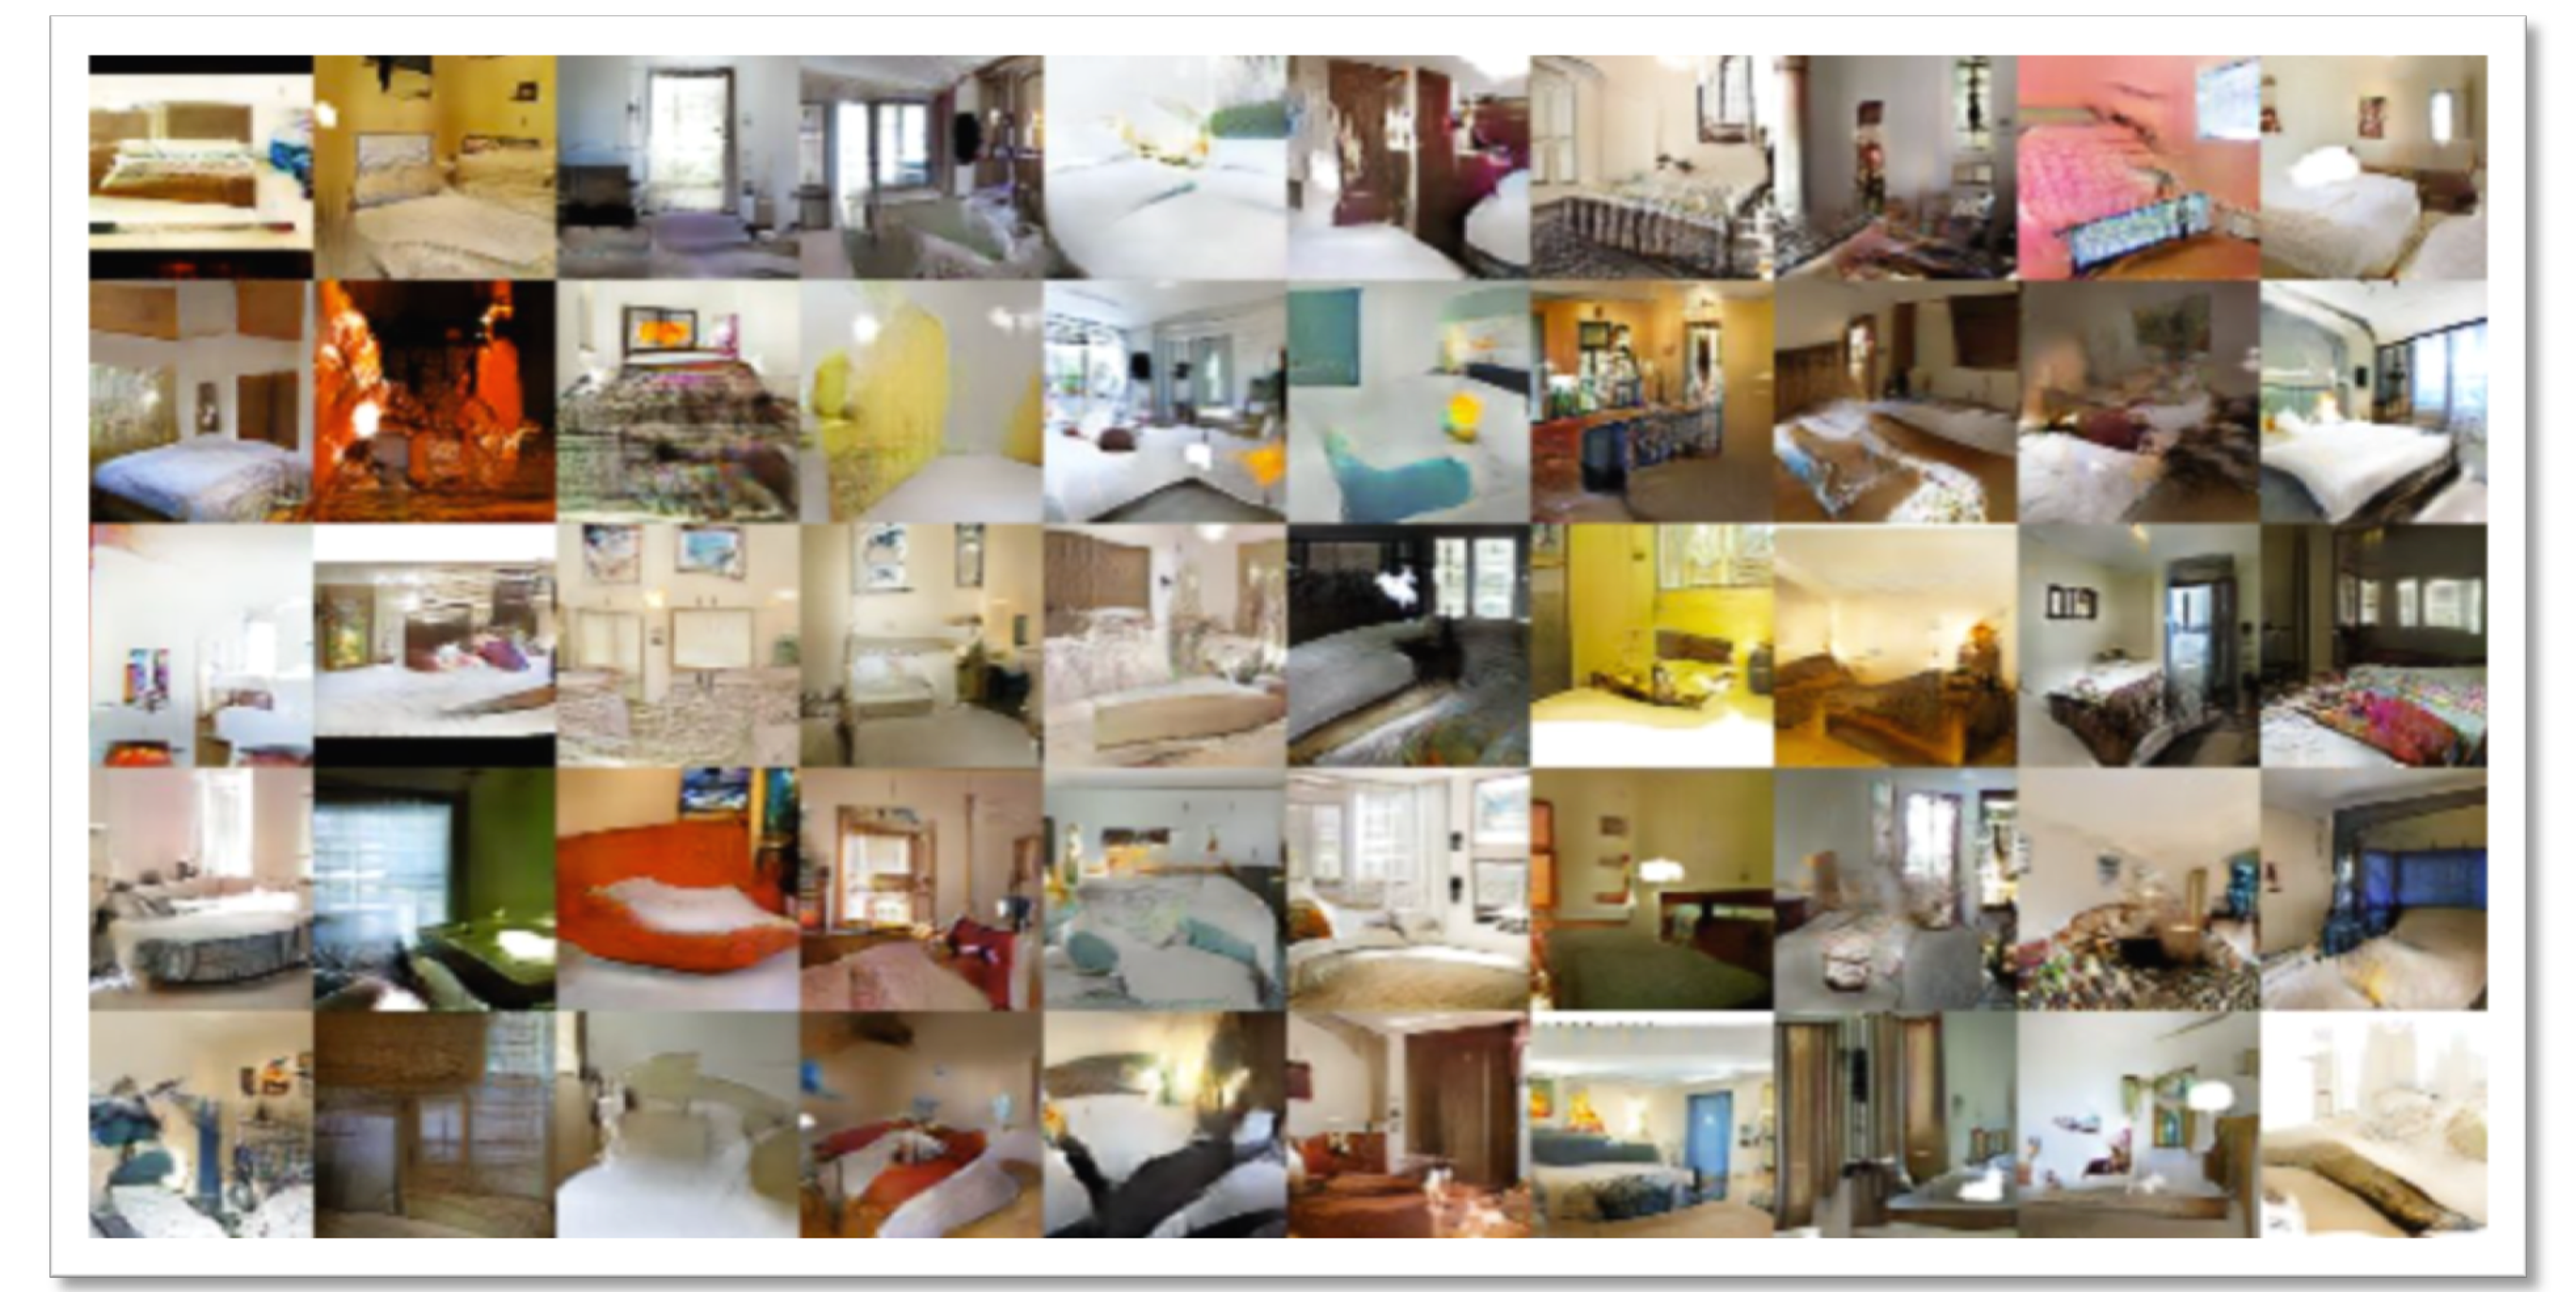
\includegraphics[width=.45\textwidth]{ganimg}}%
	\hspace{2em}%
	\subcaptionbox{图像插值\label{fig:ganinter}}
	{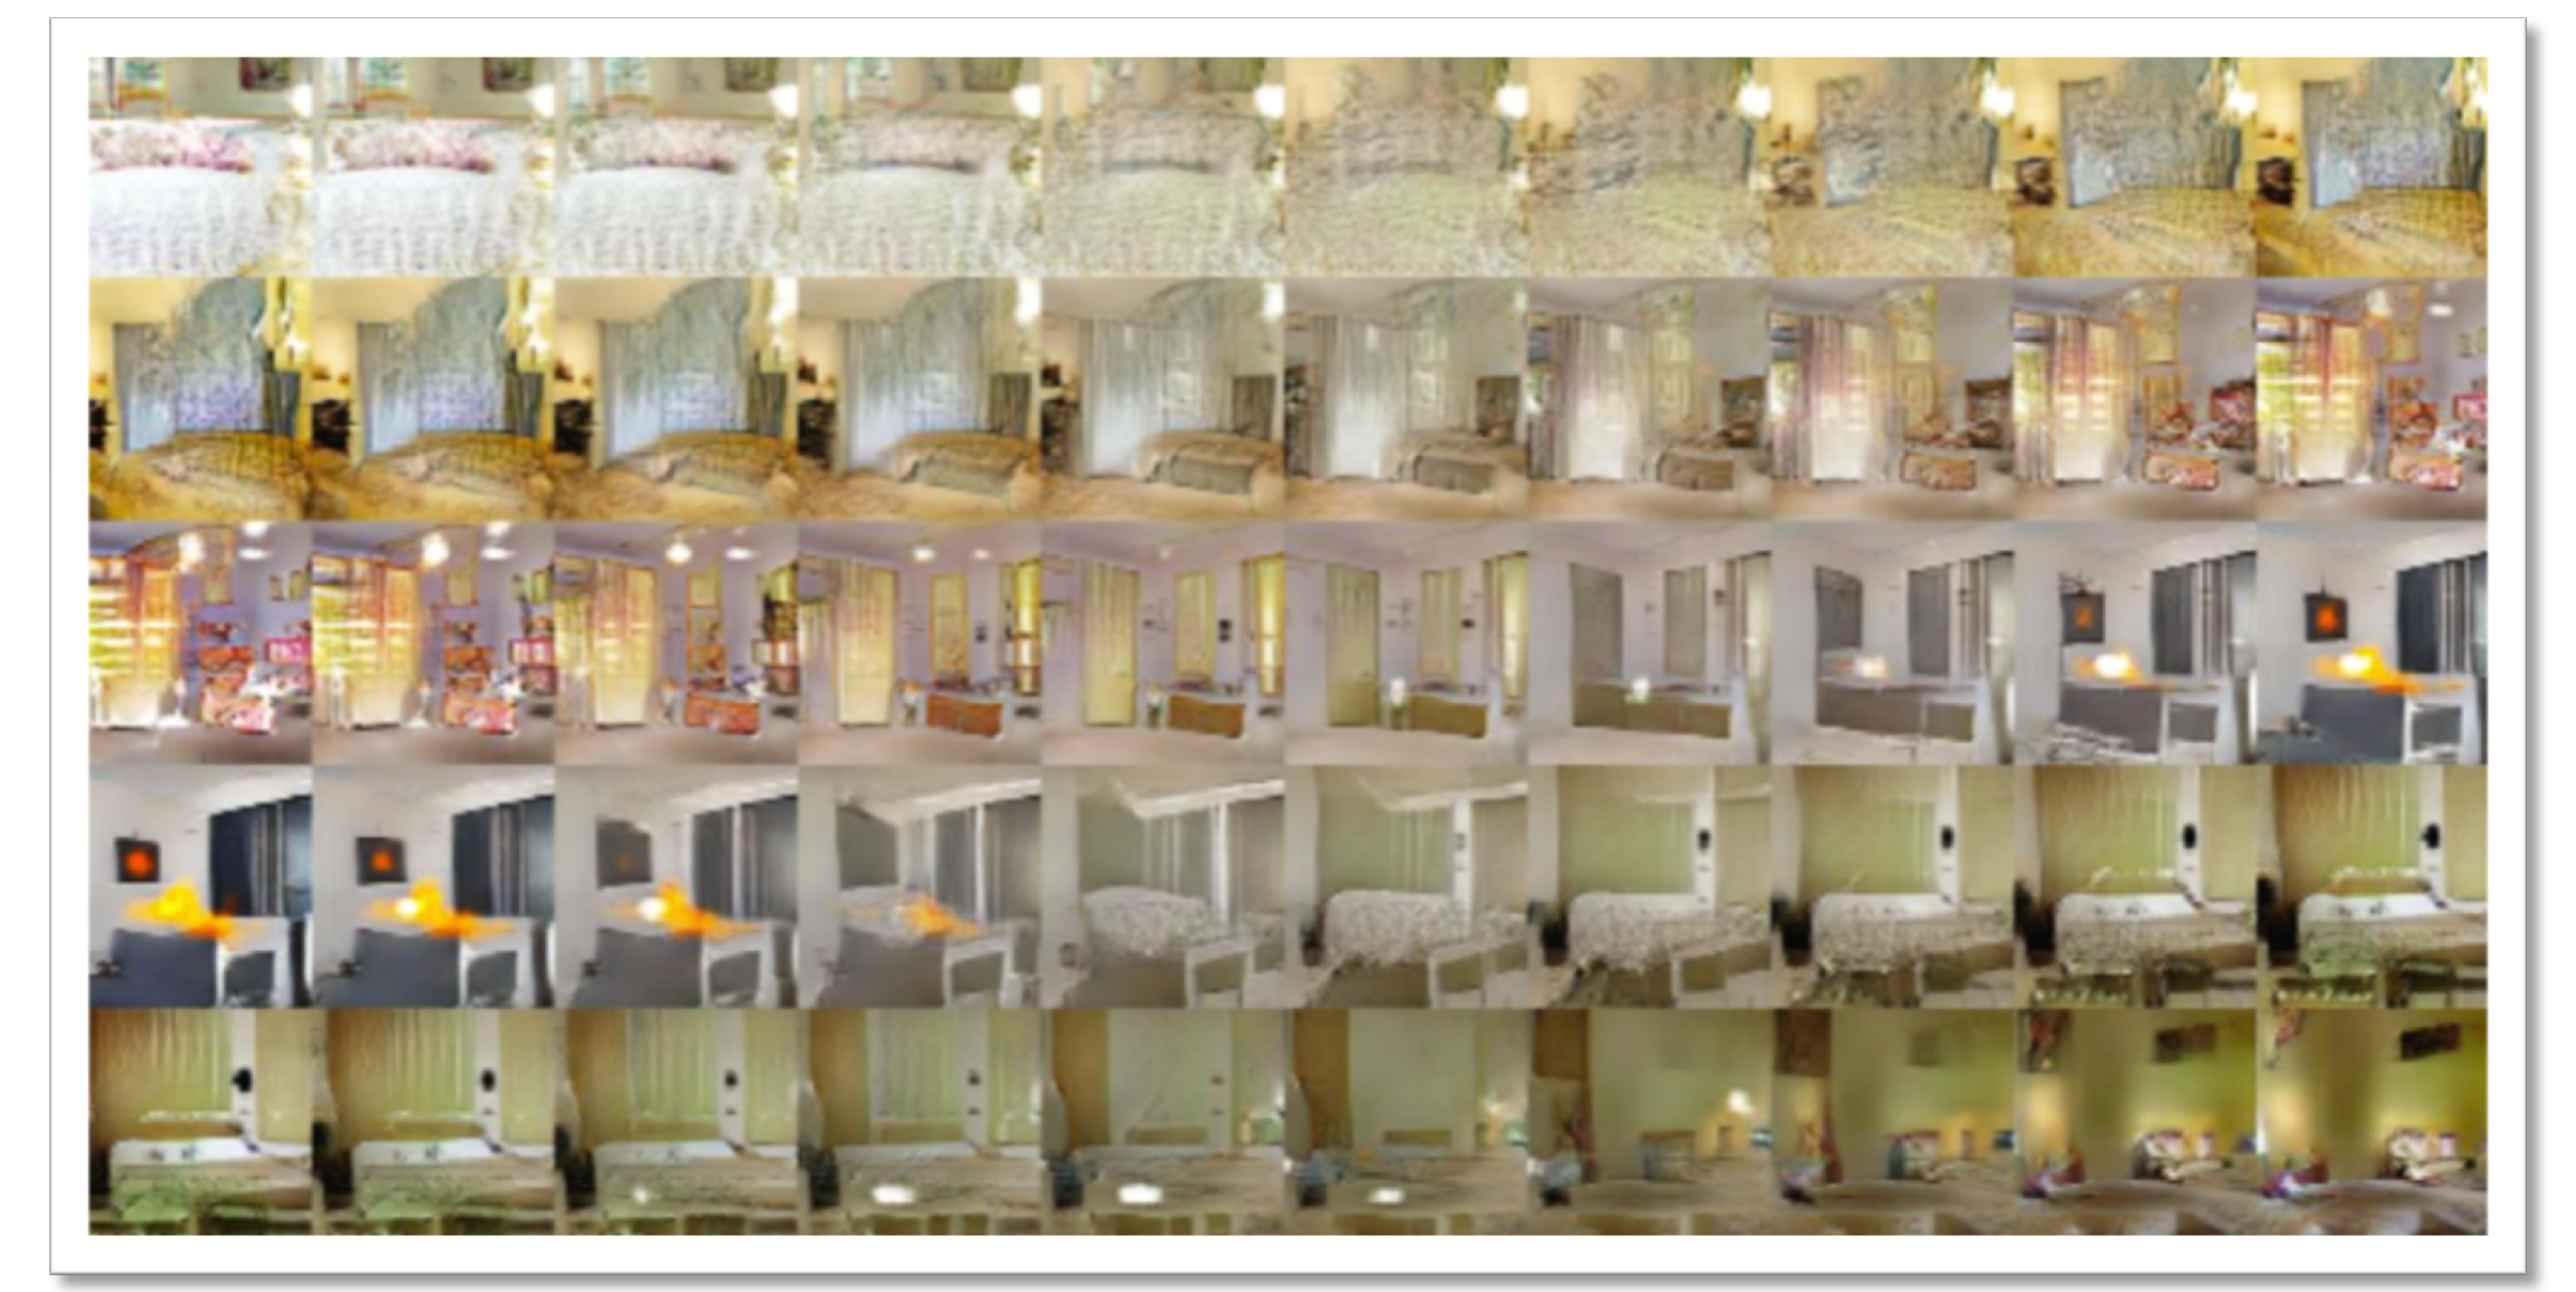
\includegraphics[width=.45\textwidth]{ganinter}}
	\caption{使用 GAN 解决图像生成任务\cite{dcgan}}
\end{figure}

尽管如此,GAN 却有训练困难、不稳定的问题。
此外,
在一些极端情况下,$G$ 还有可能会陷入只能生成一个样本或多个样本的状态,如图 \ref{fig:ganmodecollapse} 所示。
这种现象被称为模式坍塌。
我们将在第 \ref{section:ganimprove}、\ref{section:vaegan} 节中%详细
分别讨论现有研究是如何提升 GAN 的稳定性并解决模式坍塌问题的。

\begin{figure}[h]
	\centering%
	{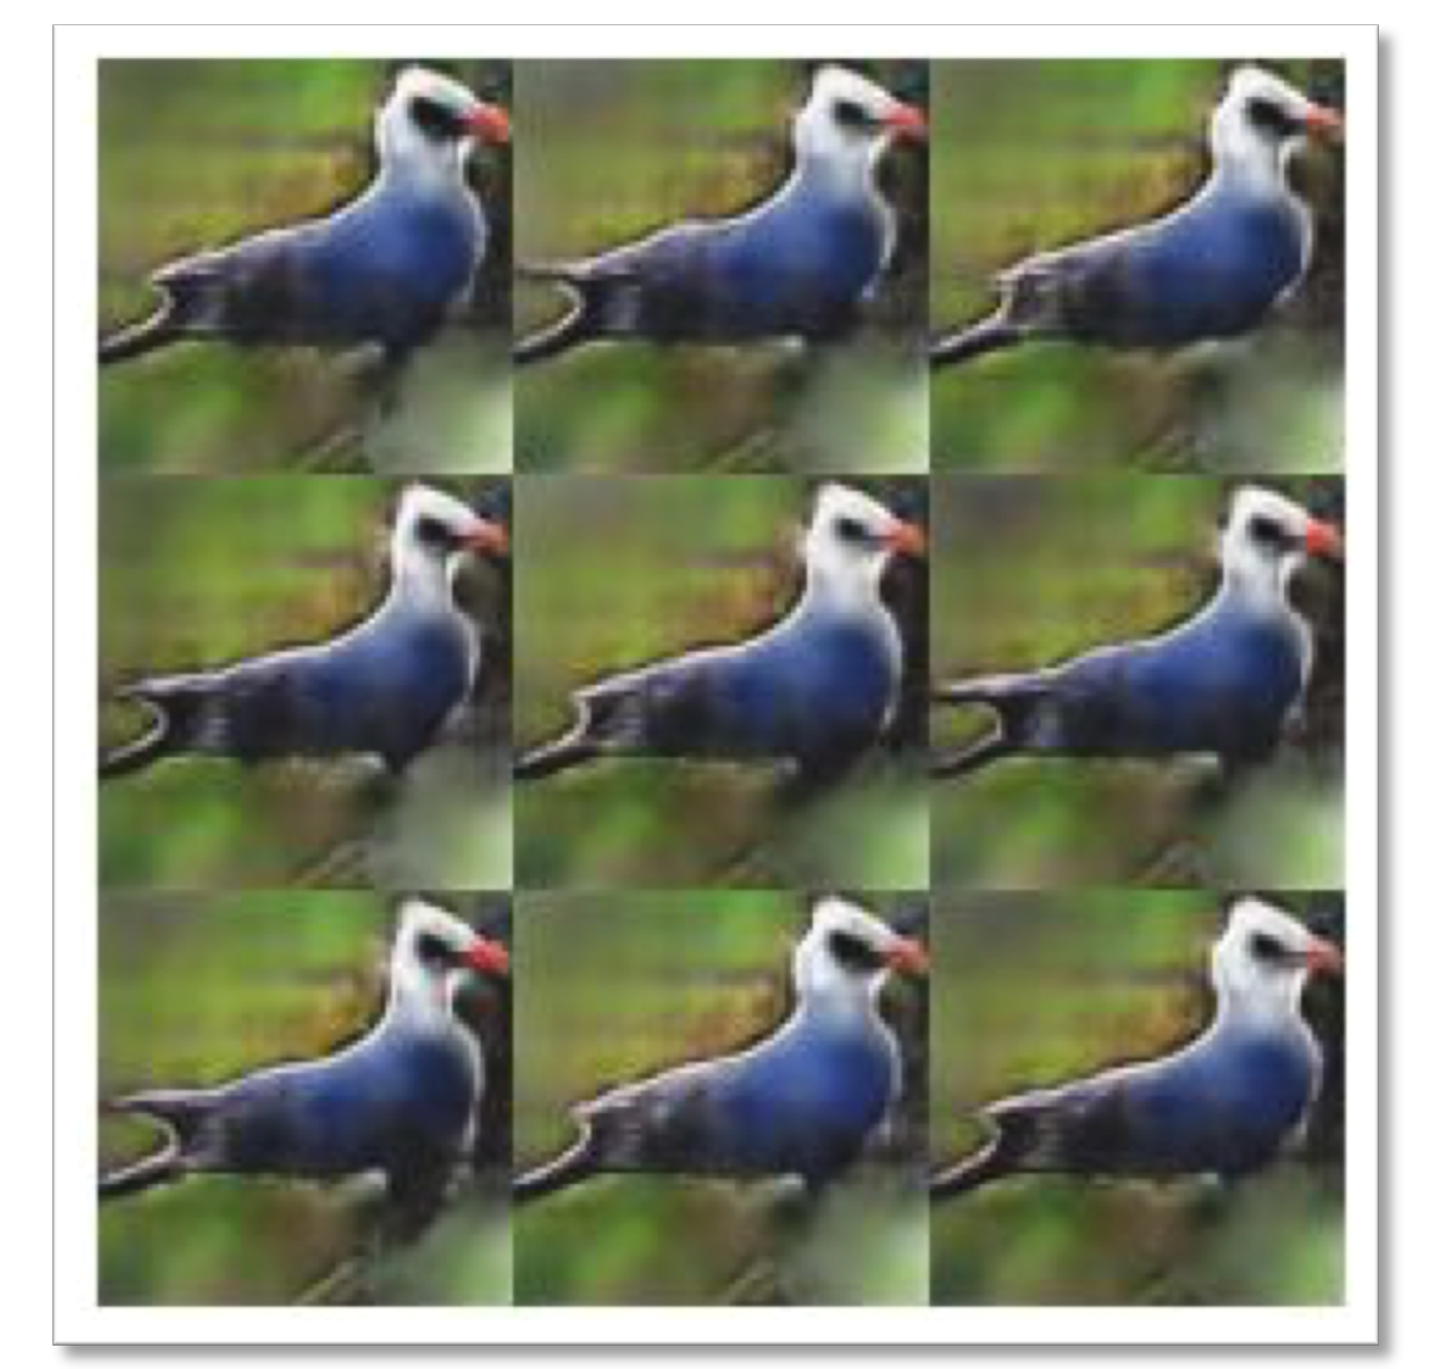
\includegraphics[width=.3\textwidth]{ganmodecollapse}}%
	\caption{GAN 的模式坍塌问题}\label{fig:ganmodecollapse}
\end{figure}
%,因为 GAN 的稳定性对 $D, G$ 的架构设计和超参数的选择非常敏感。

\section{改进 GAN 的稳定性:梯度惩罚和正则化方法 \label{section:ganimprove}}
GAN 的稳定性对 $D, G$ 的架构和超参数非常敏感,只有精心设计与选择它们,才可以得到较好的结果\cite{dcgan}。那么,导致 GAN 不稳定的原因是什么呢?

文献 \inlinecite{wganbefore} 指出:当判别器网络 $D$
达到最优状态 $D(\bm x; \bm\theta_D^*) = \PDATA(\bm x)/(\PDATA(\bm x) + \PMODEL(\bm x))$时,
式 \eqref{eq:ganloss} 可进一步简化为
\begin{align}
	\Loss(\bm\theta_G, \bm\theta_D^*) = 2\log 2 - 2 \DJS{\PDATA}{\PMODEL} \label{eq:ganlossjs}
\end{align}
此时,如果 $\PDATA(\bm x)$ 和 $\PMODEL(\bm x)$ 的支撑集之交为零测度集,那么可以证明 $\DJS{\PDATA}{\PMODEL} \equiv \log 2$,即
\begin{align}
	\Loss(\bm\theta_G, \bm\theta_D^*) \equiv 0 \label{eq:nograd}
\end{align}
这意味着生成器网络 $G$ 不能从损失函数中获取有效的梯度信息,即 $G$ 不知道如何调整决策 $\bm\theta_G$ 来降低自己的损失,训练过程就此终止。这种现象被称为梯度消失或者梯度弥散。

% 近年来,GAN的稳定训练一直是研究人员尝试攻克的重点问题。
实际上,由于 $\bm z$ 的维数通常远远低于 $G(\bm z)$ 的维数,而数据 $\bm x$ 如图像等均有信息冗余,故
$\PDATA(\bm x), \PMODEL(\bm x)$ 的支撑集都是高维空间中低维流形。在初始化阶段,其交集为零测度集的概率是 $100\%$!
因此,文献 \inlinecite{wganbefore} 中假设是绝非毫无根据、信口开河。%信口雌黄、危言耸听。%,其发生的概率是 $100\%$。

综上所述,在 $D$ 学习得
%的表现
相对较好的时候,$G$ 很有可能不知道如何调整 $\bm\theta_G$,以改善自己的表现。
要稳定训练 GAN,我们不得不平衡好 $D, G$ 的训练程度。这是导致 GAN 训练困难、
不稳定的根本原因。

为了改善 GAN 的稳定性,一种可行的方案是更改 \eqref{eq:ganloss},使得等价的优化目标不再是 $\PDATA$ 和 $\PMODEL$ 之间的散度,而是某种积分概率度量 (Integral Probability Metric, IPM),如 Wasserstein 距离\cite{wgan, wgangp} 等。这使得 $\Loss(\bm\theta_G, \bm\theta_D^*)$ 不再为恒定常数,其梯度信息可以被 $G$ 有效获取。

%,即使 $\bm\theta_G, \bm\theta_D$ 的支撑集之交为零测度集。

一些近期的研究\cite{ganestimation, lsgan2}则建议采用另一种方案:限制 $D(\bm x; \bm\theta_D)$ 必须满足 $K$-Lipschitz 连续条件。容易发现,一旦对 $D$ 施加上述限制,由 Lipschitz 连续的定义 \eqref{eq:lip},$D$ 就不再具备达到最优状态 $D(\bm x; \bm\theta_D^*)$ 的条件,式 \eqref{eq:ganlossjs}及其推论均不再成立。
\inlinecite{lsgan2} 进一步证明了,Lipschitz 连续条件能够使得训练过程有效收敛。
而按照限制 $D$ 的具体实现方案,这些工作可以被进一步分类为梯度惩罚\cite{wgangp, lsgan2, dragan}和正则化方法\cite{wgan, orthogan, sngan} 两类。




% VAE-GAN

\section{避免 GAN 的模式坍塌:VAE/GAN \label{section:vaegan}}
在第 \ref{section:gan} 节中,我们介绍了 GAN 的模式坍塌问题。但反观 VAE,我们从未发现类似的问题。
事实上,VAE 的重建误差项 \eqref{eq:vaerecons} 确保了 VAE 不会发生模式坍塌。

既然 GAN 能够生成以假乱真的高质量样本,而 VAE 又有效避免模式坍塌,那么我们可否可以取长补短,将这两者结合起来呢?
文献 \inlinecite{vaegan, cvaegan} 的工作正是这样的尝试。

我们将第 \ref{section:vae} 节介绍的 VAE 和
第 \ref{section:gan} 节介绍的 GAN 结合起来,同时合并 VAE 的解码器网络 $E$ 的 GAN 的生成器网络 $G$,
就得到了 VAE/GAN,如图\ref{fig:vaegan} 所示。
\begin{figure}[h]
	\centering%
	\subcaptionbox{网络架构\label{fig:vaegan}}
	{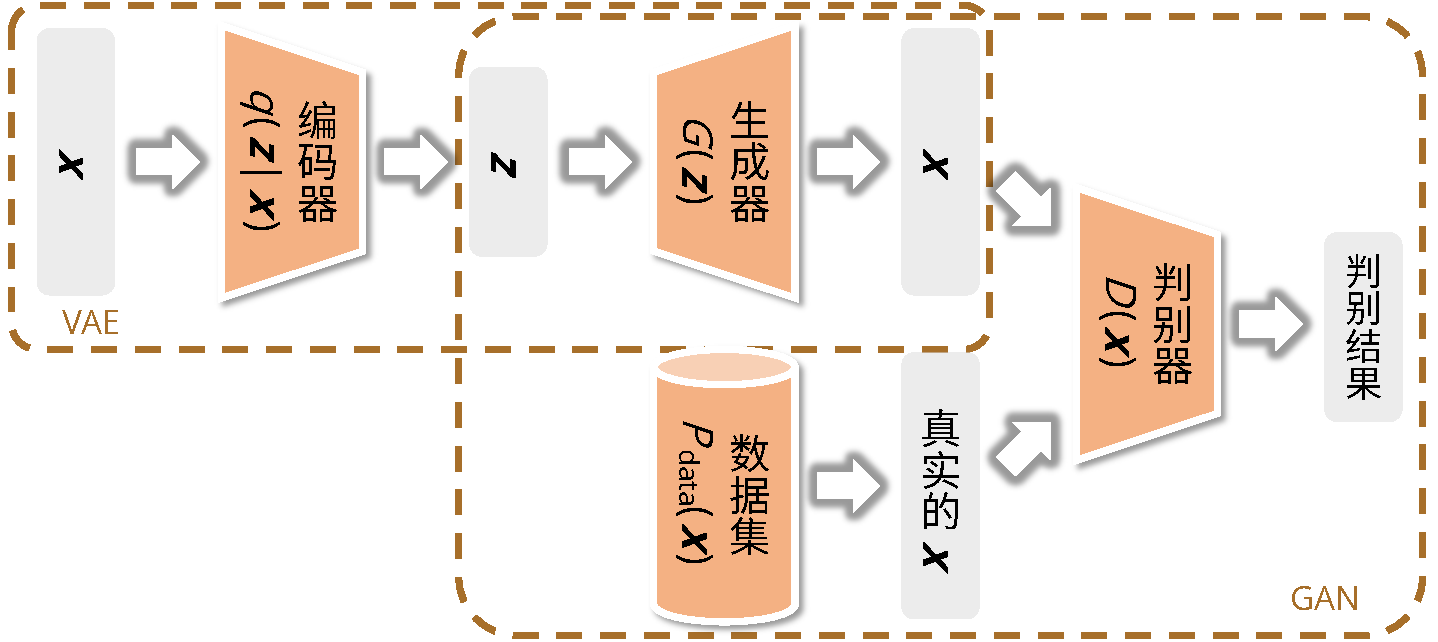
\includegraphics[width=.45\textwidth]{vaegan}}%
	\hspace{2em}%
	\subcaptionbox{损失函数\label{fig:vaeganloss}}
	{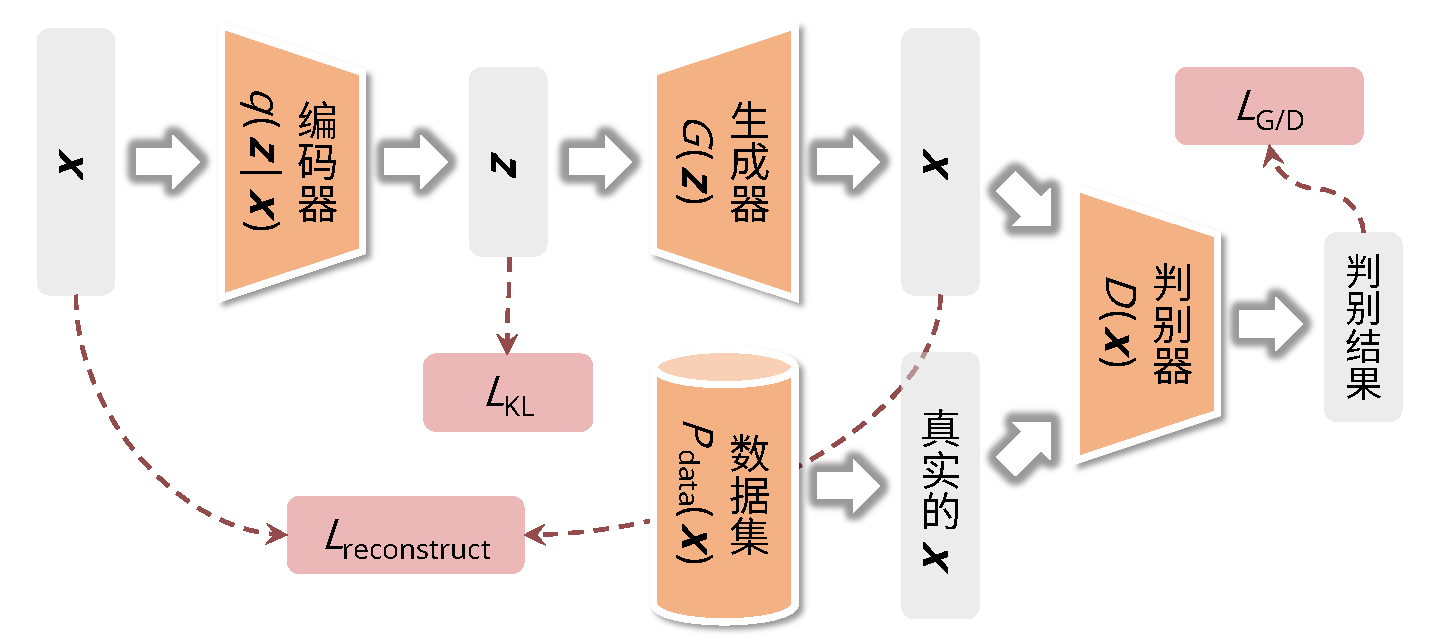
\includegraphics[width=.45\textwidth]{vaeganloss}}
	\caption{VAE/GAN\cite{vaegan}}
\end{figure}

与 VAE 和 GAN 类似,VAE/GAN 的损失函数包括三部分,分别为 KL 散度损失 $\Loss_{\text{KL}}$ 、 重建损失
$\Loss_{\text{reconstruct}}$ 以及 GAN 损失 $\Loss_{{G/D}}$:
\begin{subequations}
	\begin{align}
		\Loss_{\text{KL}}          & = \DKL{q(\bm z | \bm x; \bm\phi)}{p(\bm z)}
		\\
		\Loss_{\text{reconstruct}} & = \EXPECT{\bm z\sim q(\bm z | \bm x; \bm \phi)}{\left[\Norm*{\bm x - G(\bm z; \bm \theta)}^2\right]}
		\\
		\Loss_D                    & =
		- \EXPECT{\bm x \sim \PDATA(\bm x)}           \log(    D(\bm x))
		- \EXPECT{\bm z \sim \NormDist(\bm 0, \bm I)} \log(1 - D( G(\bm z)))
		\\
		\Loss_G                    & =
		- \EXPECT{\bm z \sim \NormDist(\bm 0, \bm I)} \log(D( G(\bm z)))
	\end{align}
	\label{eq:vaeganloss}
\end{subequations}
训练时,我们需要交替优化
\begin{subequations}
	\label{eq:vaegantrain}
	\begin{align}
		\bm\theta_D^*    & = \argmin{\bm\theta_D} = \lambda_D \cdot \Loss_D\label{eq:vaegantrain1}
		\\
		\bm\theta_\phi^* & = \argmin{\bm\theta_\phi} =
		\lambda_{\text{KL}} \cdot \Loss_{\text{KL}} +
		\lambda_{\text{reconstruct}} \cdot \Loss_{\text{reconstruct}}\label{eq:vaegantrain2}
		\\
		\bm\theta_G^*    & = \argmin{\bm\theta_G} =
		\lambda_G \cdot \Loss_G +
		\lambda_{\text{reconstruct}} \cdot \Loss_{\text{reconstruct}}\label{eq:vaegantrain3}
	\end{align}
\end{subequations}
其中 $\lambda_{\text{KL}}, \lambda_{\text{reconstruct}}, \lambda_D, \lambda_G$ 为平衡因子。
训练结束后,我们即丢弃判别器网络 $D$,与 GAN 的流程相同。


VAE/GAN 在图像生成任务上的表现如图 \ref{fig:vaegangen} 所示。
值得注意的是,由于编码器网络 $q(\bm z | \bm x)$ 可以
由数据 $\bm x$ 推出 $\bm z$ 的后验分布,因此 VAE/GAN 还可以用来
对图像进行重建或者去噪,如图  \ref{fig:vaeganrecon} 所示。
% 除了能生成图像外,GAN 还可以对图像进行插值。如图 \ref{fig:ganinter} 所示。
\begin{figure}[h]
	\centering%
	\subcaptionbox{图像生成\label{fig:vaegangen}}
	{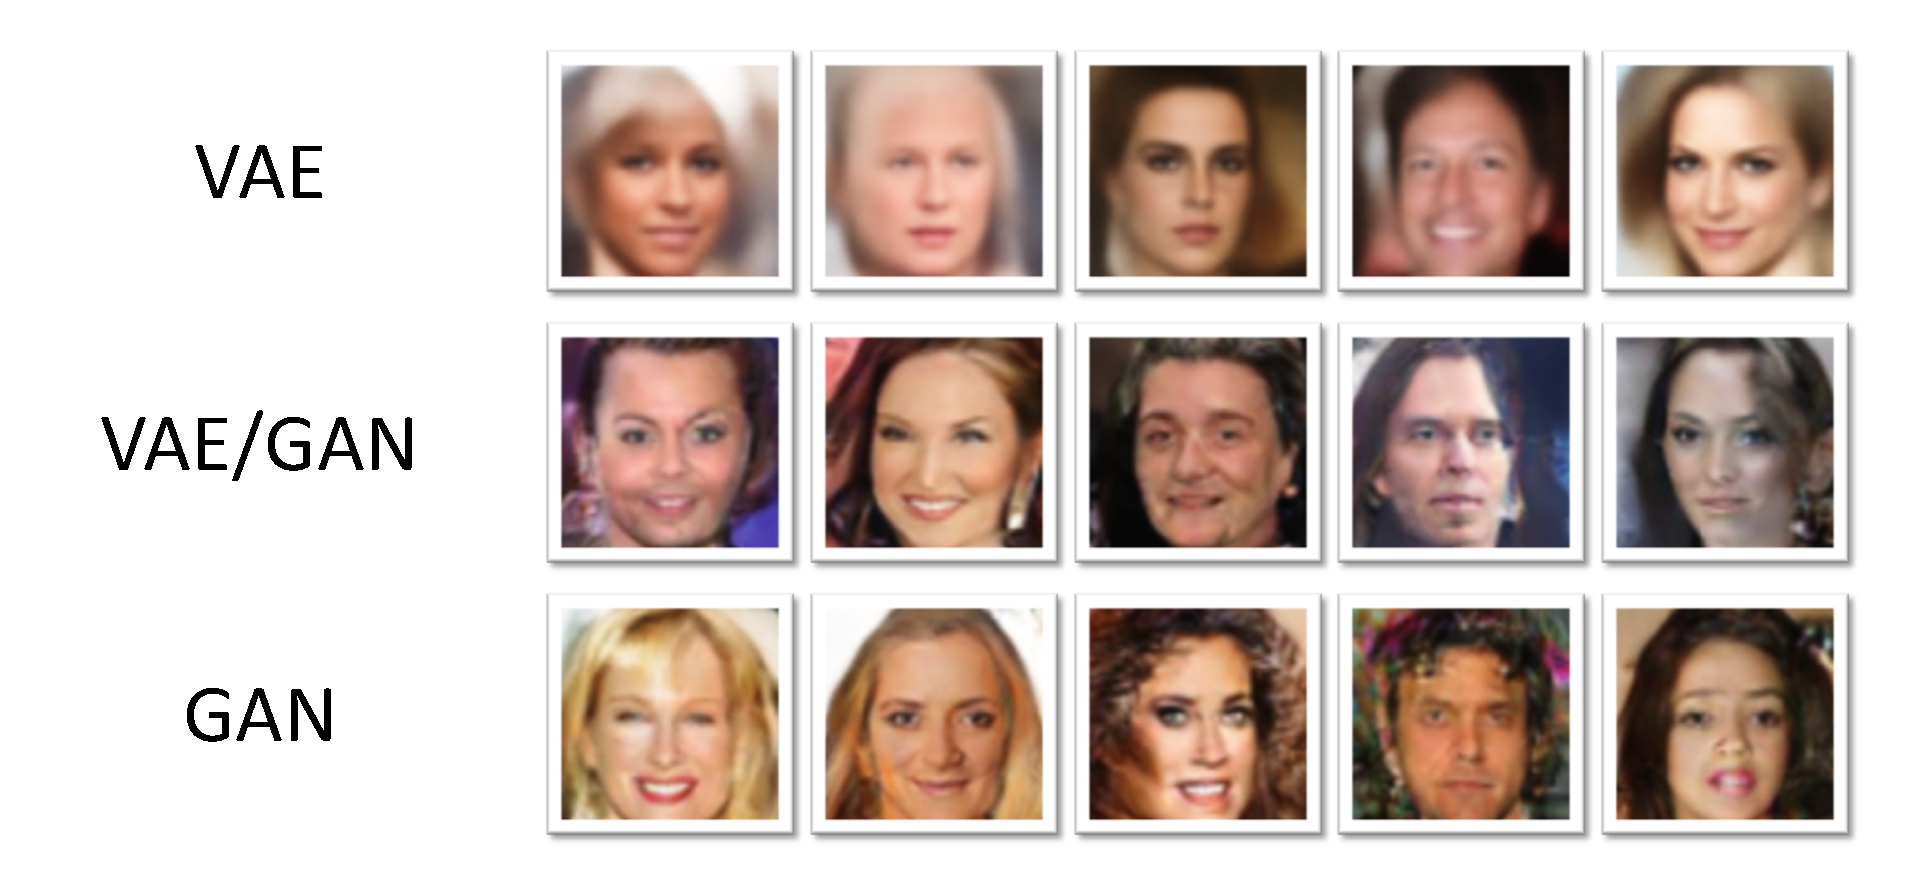
\includegraphics[width=.49\textwidth]{vaegangen}}%
	%\hspace{2em}%
	\subcaptionbox{图像重建/图像去噪\label{fig:vaeganrecon}}
	{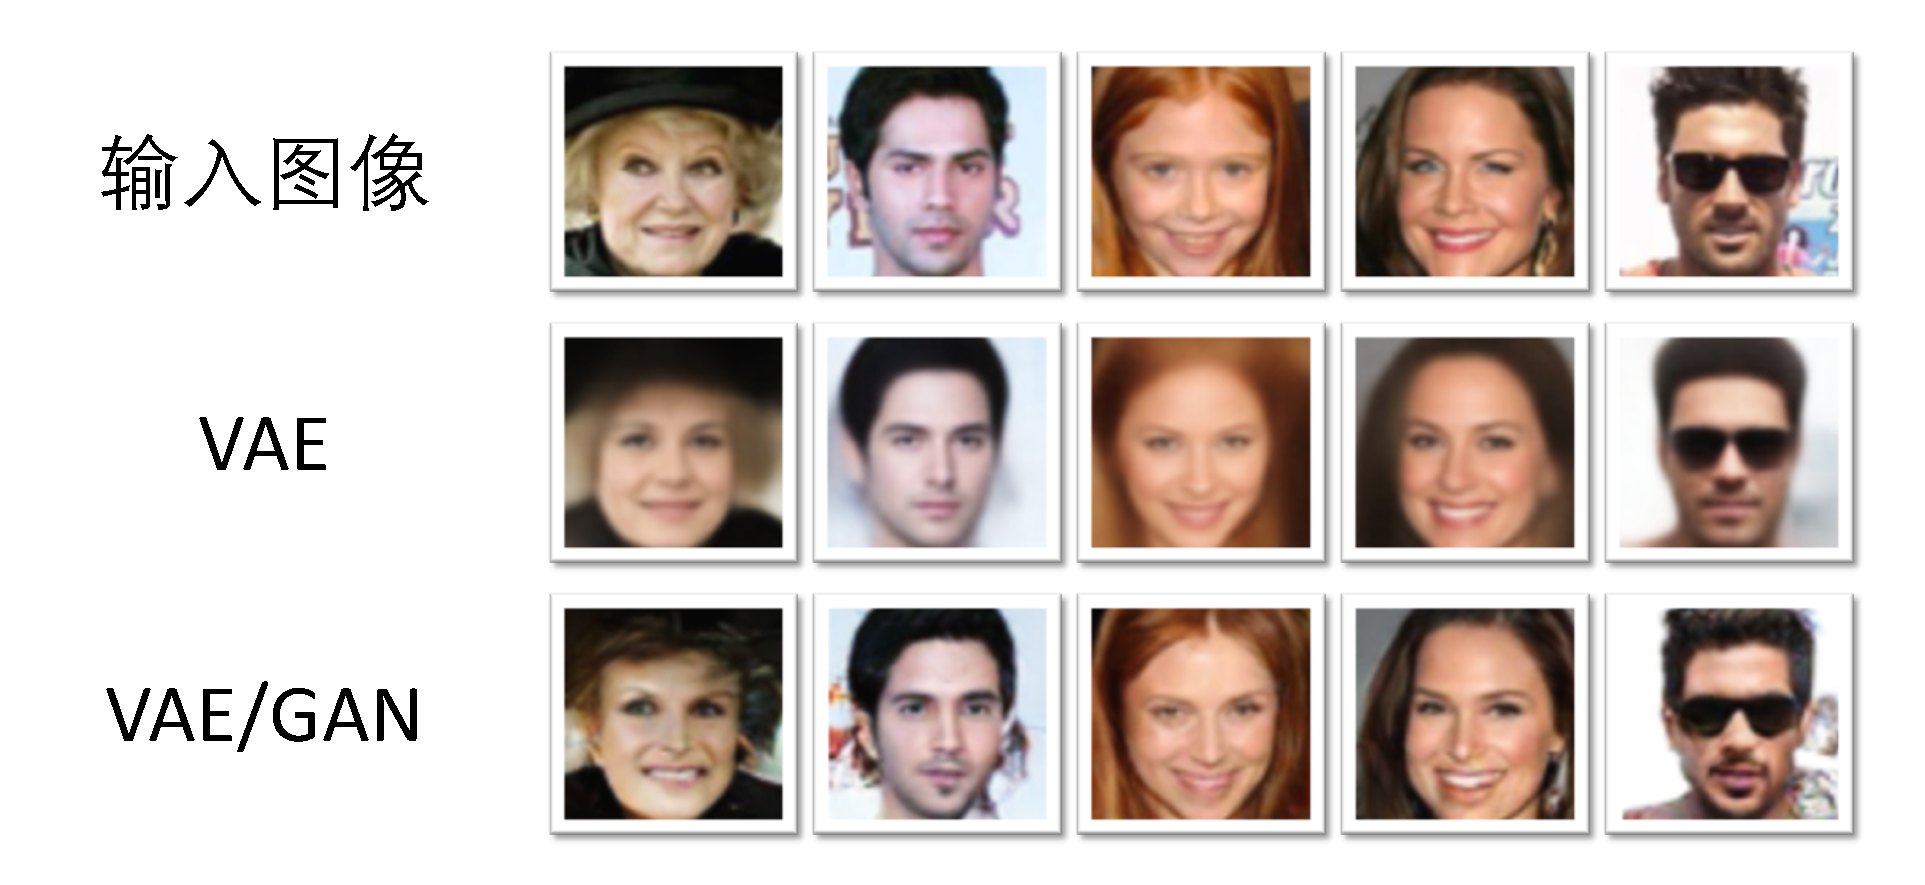
\includegraphics[width=.49\textwidth]{vaeganrecon}}
	\caption{使用 VAE/GAN 解决图像任务\cite{vaegan}}
\end{figure}

如果进一步在 VAE/GAN 中加入分类器,就可以得到 CVAE-GAN\cite{cvaegan}。它的表现效果更好,如图 \ref{fig:2dgen} 所示。限于篇幅,我们不再进一步展开介绍这个工作。


